\documentclass[polish,envcountsect,10pt]{beamer}
\usetheme{metropolis}
\usepackage[T1]{fontenc}
\usepackage{polski}
\usepackage{babel}
\usepackage{tikz}
\usepackage{graphicx}
\usepackage{xcolor}
\usepackage{algorithm}
\usepackage{algpseudocode}
\graphicspath{ {./img/} }

\title{Triangulacja i diagramy Voronoi}
\author{Krzysztof Nasuta}
\date{Gdańsk, 2025}

\begin{document}

\frame{\titlepage}

% Triangulacja w geometrii

\begin{frame}
  \frametitle{Triangulacja w geometrii}
  \begin{definition}
    Sympleks to uogólnienie trójkąta i czworościanu na dowolne wymiary. Są to najprostsze możliwe obiekty geometryczne w danym wymiarze.
  \end{definition}

  \pause
  Dla przykładu:
  \begin{itemize}
    \item 0-wymiarowy sympleks to punkt,
    \item 1-wymiarowy sympleks to odcinek,
    \item 2-wymiarowy sympleks to trójkąt,
    \item 3-wymiarowy sympleks to czworościan,
  \end{itemize}
\end{frame}

\begin{frame}
  \frametitle{Triangulacja w geometrii}
  \begin{definition}
    Triangulacja to podział płaszczyzny euklidesowej na trójkąty. W ogólności mówi się o podziale przestrzeni euklidesowej na sympleksy odpowiedniego wymiaru.

    \pause
    Zazwyczaj wymagane jest, aby krawędzie i wierzchołki sympleksów pokrywały się w całości z krawędziami i wierzchołkami innych sympleksów.
  \end{definition}
\end{frame}

\begin{frame}
  \frametitle{Triangulacja w geometrii - przykład dwuwymiarowy}
  \begin{center}
    \begin{figure}
      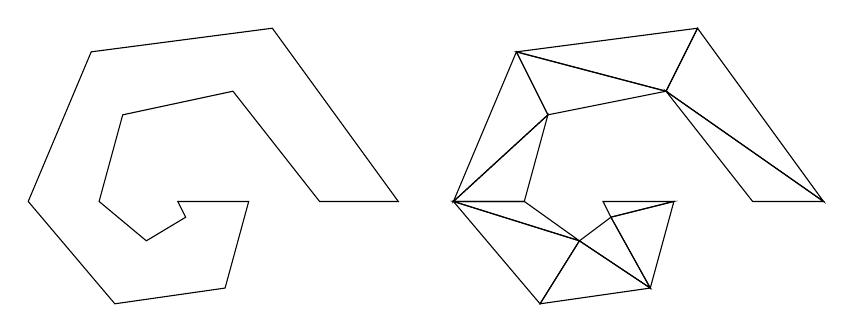
\begin{tikzpicture}
        \draw (1.3, 1.5) -- (1.6, 2.6) -- (3.0, 2.9) -- (4.1, 1.5) -- (5.1, 1.5) -- (3.5, 3.7) -- (1.2, 3.4) -- (0.4, 1.5) -- (1.5, 0.2) -- (2.9, 0.4) -- (3.2, 1.5) -- (2.3, 1.5) -- (2.4, 1.3) -- (1.9, 1.0) -- cycle;

        \pause
        \draw (7.8, 1.3) -- (7.4, 1.0) -- (8.3, 0.4) -- cycle;
        \draw (7.8, 1.3) -- (8.3, 0.4) -- (8.6, 1.5) -- cycle;
        \draw (7.8, 1.3) -- (8.6, 1.5) -- (7.7, 1.5) -- cycle;
        \draw (6.9, 0.2) -- (8.3, 0.4) -- (7.4, 1.0) -- cycle;
        \draw (6.9, 0.2) -- (7.4, 1.0) -- (5.8, 1.5) -- cycle;
        \draw (5.8, 1.5) -- (7.4, 1.0) -- (6.7, 1.5) -- cycle;
        \draw (5.8, 1.5) -- (6.7, 1.5) -- (7.0, 2.6) -- cycle;
        \draw (5.8, 1.5) -- (7.0, 2.6) -- (6.6, 3.4) -- cycle;
        \draw (7.0, 2.6) -- (8.5, 2.9) -- (6.6, 3.4) -- cycle;
        \draw (9.6, 1.5) -- (10.5, 1.5) -- (8.5, 2.9) -- cycle;
        \draw (8.9, 3.7) -- (6.6, 3.4) -- (8.5, 2.9) -- cycle;
        \draw (8.9, 3.7) -- (8.5, 2.9) -- (10.5, 1.5) -- cycle;
      \end{tikzpicture}
      \caption{Podział płaszczyzny na trójkąty}
    \end{figure}
  \end{center}
\end{frame}

\begin{frame}
  \frametitle{Triangulacja w geometrii - przykład trójwymiarowy}
  \begin{center}
    \begin{figure}
      \includegraphics[scale=0.5]{3d-triangulation}
      \caption{Podział bryły na czworościany}
    \end{figure}
  \end{center}
\end{frame}

\begin{frame}
  \frametitle{Triangulacja w teorii grafów}
  \begin{definition}
    Graf planarny to graf, który można narysować na płaszczyźnie w taki sposób, że jego krawędzie nie przecinają się ze sobą.
  \end{definition}

  \begin{example}
    \begin{center}
      \begin{figure}
        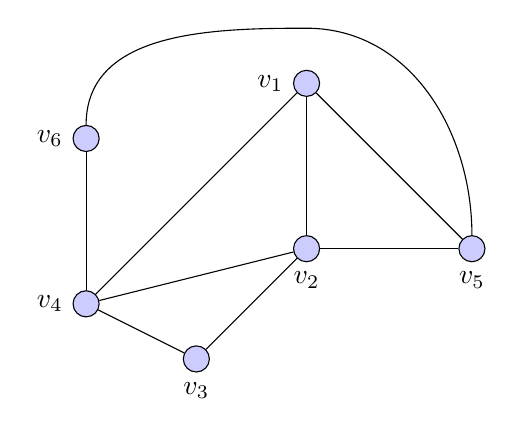
\begin{tikzpicture}[scale=0.7]
          \node[circle, draw, fill=blue!20, label=left:{$v_1$}] (v1) at (2,3) {};
          \node[circle, draw, fill=blue!20, label=below:{$v_2$}] (v2) at (2,0) {};
          \node[circle, draw, fill=blue!20, label=below:{$v_3$}] (v3) at (0,-2) {};
          \node[circle, draw, fill=blue!20, label=left:{$v_4$}] (v4) at (-2,-1) {};
          \node[circle, draw, fill=blue!20, label=below:{$v_5$}] (v5) at (5,0) {};
          \node[circle, draw, fill=blue!20, label=left:{$v_6$}] (v6) at (-2,2) {};

          \coordinate (ctrl-5-6) at (2,4);

          \draw (v1) -- (v2);
          \draw (v1) -- (v5);
          \draw (v2) -- (v3);
          \draw (v2) -- (v4);
          \draw (v2) -- (v5);
          \draw (v3) -- (v4);
          \draw (v4) -- (v1);
          \draw (v4) -- (v6);
          \draw (v5) to[out=90, in=0] (ctrl-5-6) to[out=180, in=90] (v6);
        \end{tikzpicture}
        \caption{Przykład grafu planarnego}
      \end{figure}
    \end{center}
  \end{example}
\end{frame}

\begin{frame}
  \frametitle{Triangulacja w teorii grafów}
  \begin{definition}
    Maksymalny graf planarny to \textbf{graf planarny, do którego nie można dodać żadnej krawędzi bez utraty własności planarnych}. W maksymalnym grafie planarnym każda ściana jest trójkątem (wliczając ścianę zewnętrzną).
  \end{definition}

  \pause
  \begin{definition}
    Triangulacja to \textbf{proces tworzenia grafu maksymalnie planarnego ze zbioru punktów}.
  \end{definition}

  \pause
  \begin{theorem}
    Jeśli maksymalny graf planarny ma $n$ wierzchołków, gdzie $n \geq 3$, to ma dokładnie $3n - 6$ krawędzi i $2n - 4$ ścian. \qed
  \end{theorem}
\end{frame}

\begin{frame}
  \frametitle{Triangulacja w teorii grafów - przykład}
  \begin{center}
    \begin{figure}
      \begin{tikzpicture}[scale=0.5]
        \node[circle, draw, fill=blue!20, label=left:{$v_1$}] (v1) at (0,5) {};
        \node[circle, draw, fill=blue!20, label=right:{$v_2$}] (v2) at (0,0) {};
        \node[circle, draw, fill=blue!20, label=left:{$v_3$}] (v3) at (0,-5) {};
        \node[circle, draw, fill=blue!20, label=above:{$v_4$}] (v4) at (2,2) {};
        \node[circle, draw, fill=blue!20, label=below:{$v_5$}] (v5) at (2,-2) {};
        \node[circle, draw, fill=blue!20, label=right:{$v_6$}] (v6) at (-2,2) {};
        \node[circle, draw, fill=blue!20, label=left:{$v_7$}] (v7) at (-2,-2) {};
        \node[circle, draw, fill=blue!20, label=below:{$v_8$}] (v8) at (-6,0) {};
        \node[circle, draw, fill=blue!20, label=below:{$v_9$}] (v9) at (6,0) {};
        \node[circle, draw, fill=blue!20, label=below:{$v_{10}$}] (v10) at (-9,0) {};
        \node[circle, draw, fill=blue!20, label=below:{$v_{11}$}] (v11) at (9,0) {};

        \coordinate (ctrl-1-3) at (11, 0);

        \pause
        \draw (v1) -- (v6);
        \pause
        \draw (v1) -- (v2);
        \draw (v2) -- (v6);
        \pause
        \draw (v1) to[out=0, in=90] (ctrl-1-3) to[out=-90, in=0] (v3);
        \draw (v1) -- (v4);
        \draw (v1) -- (v8);
        \draw (v1) -- (v9);
        \draw (v1) -- (v10);
        \draw (v1) -- (v11);
        \draw (v2) -- (v3);
        \draw (v2) -- (v4);
        \draw (v2) -- (v5);
        \draw (v2) -- (v7);
        \draw (v2) -- (v8);
        \draw (v2) -- (v9);
        \draw (v3) -- (v5);
        \draw (v3) -- (v7);
        \draw (v3) -- (v8);
        \draw (v3) -- (v9);
        \draw (v3) -- (v10);
        \draw (v3) -- (v11);
        \draw (v4) -- (v9);
        \draw (v5) -- (v9);
        \draw (v6) -- (v8);
        \draw (v7) -- (v8);
        \draw (v8) -- (v10);
        \draw (v9) -- (v11);

        \pause
        \draw[fill=blue!30, draw=black] (0,5) -- (0,0) -- (-2,2) -- cycle;
        \node[fill=white] at (0,-2) {Wszystkie ściany są trójkątami (także zewnętrzna)};
      \end{tikzpicture}
      \caption{Graf Goldnera-Harary'ego - przykład grafu maksymalnie planarnego o 11 wierzchołkach i 27 krawędziach}
    \end{figure}
  \end{center}
\end{frame}

\begin{frame}
  \frametitle{Triangulacja w teorii grafów}
  \begin{definition}
    Cykl indukowany to taki cykl w grafie, że żadne dwa jego wierzchołki nie są połączone krawędzią, która nie należy do cyklu.
  \end{definition}

  \begin{definition}
    Graf cięciwowy to graf, w którym każdy \textbf{cykl o długości czterech lub większej ma przekątną}, czyli krawędź łączącą dwa niekolejne wierzchołki cyklu.

    W grafie takim cykle indukowane mają zawsze długość 3.
  \end{definition}
  \pause
  \begin{definition}
    Triangulacja to proces dodawania krawędzi do grafu w celu \textbf{otrzymania grafu cięciwowego}.
  \end{definition}
\end{frame}

\begin{frame}
  \frametitle{Triangulacja w teorii grafów - przykład}
  \begin{center}
    \begin{figure}
      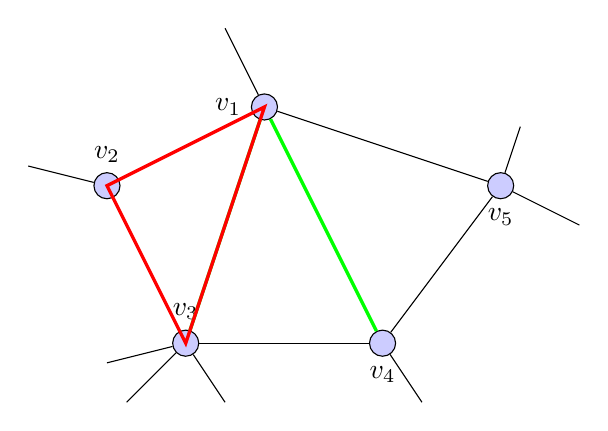
\begin{tikzpicture}[scale=1.0]
        \node[circle, draw, fill=blue!20, label=left:{$v_1$}] (v1) at (0,1) {};
        \node[circle, draw, fill=blue!20, label=above:{$v_2$}] (v2) at (-2,0) {};
        \node[circle, draw, fill=blue!20, label=above:{$v_3$}] (v3) at (-1,-2) {};
        \node[circle, draw, fill=blue!20, label=below:{$v_4$}] (v4) at (1.5,-2) {};
        \node[circle, draw, fill=blue!20, label=below:{$v_5$}] (v5) at (3,0) {};

        \draw (v1) -- (-0.5, 2);
        \draw (v1) -- (v2);
        \draw (v2) -- (-3, 0.25);
        \draw (v2) -- (v3);
        \draw (v3) -- (-2, -2.25);
        \draw (v3) -- (-1.75, -2.75);
        \draw (v3)-- (-0.5, -2.75);
        \draw (v3) -- (v4);
        \draw (v4) -- (2, -2.75);
        \draw (v4) -- (v5);
        \draw (v5) -- (4, -0.5);
        \draw (v5) -- (3.25, 0.75);
        \draw (v5) -- (v1);

        \pause
        \draw[very thick, color=green] (v1) -- (v3);
        \draw[very thick, color=green] (v1) -- (v4);

        \pause
        \draw[very thick, draw=red] (0,1) -- (-2,0) -- (-1,-2) -- cycle;

      \end{tikzpicture}
      \caption{Przykład triangulacji grafu poprzez dodanie krawędzi $(v_1, v_3)$ oraz $(v_1, v_4)$. W procesie tym powstały trzy cykle indukowane o długości 3.}
    \end{figure}
  \end{center}
\end{frame}

\begin{frame}
  \frametitle{Diagramy Voronoi}
  \begin{definition}
    Tesselacja to pokrycie płaszczyzny za pomocą wielokątów przylegających do siebie oraz nie nakładających się.
  \end{definition}

  \begin{definition}
    Diagram Voronoi to \textbf{podział płaszczyzny na obszary w oparciu o odległość do określonego zbioru punktów}. Każdy obszar składa się z punktów bliższych do jednego punktu z danego zbioru niż do jakiegokolwiek innego punktu ze zbioru. Jest to przykład tesselacji płaszczyzny.
  \end{definition}

  \pause
  Diagramy te zostały nazwane na cześć matematyka Gieorgija Woronoj'a, rosyjskiego matematyka ukraińskiego pochodzenia, który opisał je w 1908 roku.
\end{frame}

\begin{frame}
  \frametitle{Diagramy Voronoi}
  Niech $P = \{p_1, p_2, \ldots, p_n\}$, gdzie $p_i \in \mathbb{R}^2, n \in \mathbb{N}$.
  Punkty ze zbioru $P$ nazywać będziemy centrami.

  \begin{definition}
    Komórką diagramu Voronoi dla punktu $p_i$ nazywamy
    \begin{center}
      $V_P(p_i) = \{x : \forall_{j \neq i} d(x, p_i) \leq d(x, p_j) \}$
    \end{center}
    gdzie $d$ jest funkcją odległości między punktami.
  \end{definition}

  \pause
  \begin{definition}
    Podział płaszczyzny na $n$ komórek Voronoi $V_P(p_1), V_P(p_2), \ldots, V_P(p_n)$ nazywamy diagramem Voronoi dla zbioru punktów $P$. Oznaczamy go jako $Vor(P)$.
  \end{definition}
\end{frame}

\begin{frame}
  \frametitle{Diagramy Voronoi - przykład}
  \begin{center}
    \begin{figure}
      \includegraphics<1>[scale=0.4]{voronoi-animation-0}
      \includegraphics<2>[scale=0.4]{voronoi-animation-1}
      \includegraphics<3>[scale=0.4]{voronoi-animation-2}
      \caption{Przykład diagramu Voronoi dla metryki euklidesowej}
    \end{figure}
  \end{center}
\end{frame}

\begin{frame}
  \frametitle{Diagramy Voronoi - porównanie metryk}

  Do najpopularniejszych metryk używanych w diagramach Voronoi należą:
  \begin{itemize}
    \item Metryka euklidesowa \\
      $d[(a_1, a_2), (b_1, b_2)] = \sqrt{(a_1 - b_1)^2 + (a_2 - b_2)^2}$
    \item Metryka Manhattan \\
      $d[(a_1, a_2), (b_1, b_2)] = |a_1 - b_1| + |a_2 - b_2|$
    \item Metryka Czebyszewa \\
      $d[(a_1, a_2), (b_1, b_2)] = \max(|a_1 - b_1|, |a_2 - b_2|)$
  \end{itemize}
\end{frame}

\begin{frame}
  \frametitle{Diagramy Voronoi - porównanie metryk}
  \begin{center}
    \begin{figure}
      \includegraphics<1>[scale=0.35]{voronoi_euklidesowa}
      \includegraphics<2>[scale=0.35]{voronoi_manhattan}
      \includegraphics<3>[scale=0.35]{voronoi_czebyszewa}
      \only<1>{\caption{Diagram Voronoi dla metryki euklidesowej}}
      \only<2>{\caption{Diagram Voronoi dla metryki Manhattan}}
      \only<3>{\caption{Diagram Voronoi dla metryki Czebyszewa}}
    \end{figure}
  \end{center}
\end{frame}

\begin{frame}
  \frametitle{Diagramy Voronoi - algorytmy tworzenia}
  Do najpopularniejszych sposobów tworzenia diagramów Voronoi należą:
  \begin{itemize}
    \item \color<1>{violet}{\textbf{Rastrowy brute force} - dla każdej komórki siatki obliczana jest odległość do każdego punktu ze zbioru $P$, a komórka jest przypisywana do najbliższego punktu. Czas działania: $O(mn)$, gdzie $m$ to liczba komórek siatki, a $n$ to liczba punktów w zbiorze $P$.}
      \pause
    \item \color<2>{violet}{\textbf{Algorytm Fortune'a} - najczęściej stosowany, pozwala na zbudowanie diagramu Voronoi w czasie $O(n \log n)$ dla $n$ punktów wejściowych. Jest to algorytm przemiatania - linia omija zbiór punktów w określonym kierunku, a kiedy wszystkie punkty zostaną przeciągnięte, tworzony jest diagram Voronoi.}
      \pause
    \item \color<3>{violet}{\textbf{Obliczanie triangulacji Delaunaya} (\textit{Delone}) i tworzenie diagramu Vorornoi na jej podstawie. Złożoność: $O(n \log n)$.}
  \end{itemize}
\end{frame}

\begin{frame}
  \frametitle{Diagramy Voronoi - Rastrowy brute force}

  \begin{algorithm}[H]
    \caption{Rastrowy brute force dla diagramu Voronoi}
    \begin{algorithmic}
      \Function{voronoiBruteForce}{siatka, punkty}
      \For{each komórka $c$ in siatka}
      \State $minimalnyDystans \gets \infty$
      \State $najbliższyPunkt \gets null$
      \For{each punkt $p$ in punkty}
      \State $dystans \gets d(c, p)$
      \If{$dystans < minimalnyDystans$}
      \State $minimalnyDystans \gets dystans$
      \State $najbliższyPunkt \gets p$
      \EndIf
      \EndFor
      \State przypisz komórkę $c$ do $najbliższyPunkt$
      \EndFor
      \State \Return siatka
      \EndFunction
    \end{algorithmic}
  \end{algorithm}
\end{frame}

\begin{frame}
  \frametitle{Diagramy Voronoi - Rastrowy brute force}

  \begin{center}
    \begin{figure}
      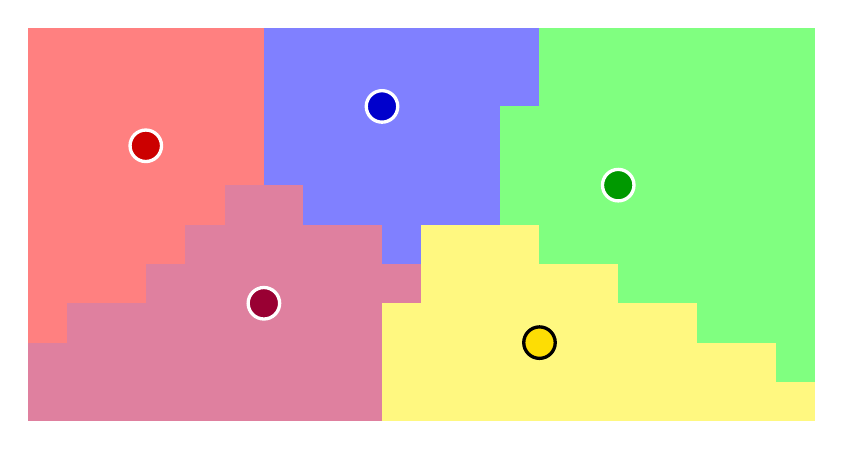
\begin{tikzpicture}[scale=0.5]
        \foreach \x in {0,1,...,19} {
          \foreach \y in {0,1,...,9} {
            \fill[gray!20] (\x, \y) rectangle (\x+1, \y+1);
          }
        }

        \foreach \x in {0,1,...,19} {
          \foreach \y in {0,1,...,9} {
            \pgfmathsetmacro{\distRed}{sqrt((\x+0.5-3)^2 + (\y+0.5-7)^2)}
            \pgfmathsetmacro{\distBlue}{sqrt((\x+0.5-9)^2 + (\y+0.5-8)^2)}
            \pgfmathsetmacro{\distGreen}{sqrt((\x+0.5-15)^2 + (\y+0.5-6)^2)}
            \pgfmathsetmacro{\distYellow}{sqrt((\x+0.5-13)^2 + (\y+0.5-2)^2)}
            \pgfmathsetmacro{\distPurple}{sqrt((\x+0.5-6)^2 + (\y+0.5-3)^2)}

            \pgfmathsetmacro{\minDist}{min(min(min(\distRed, \distBlue), min(\distGreen, \distYellow)), \distPurple)}

            \ifdim \minDist pt = \distRed pt
            \fill[red!50] (\x, \y) rectangle (\x+1, \y+1);
            \else\ifdim \minDist pt = \distBlue pt
            \fill[blue!50] (\x, \y) rectangle (\x+1, \y+1);
            \else\ifdim \minDist pt = \distGreen pt
            \fill[green!50] (\x, \y) rectangle (\x+1, \y+1);
            \else\ifdim \minDist pt = \distYellow pt
            \fill[yellow!50] (\x, \y) rectangle (\x+1, \y+1);
            \else
            \fill[purple!50] (\x, \y) rectangle (\x+1, \y+1);
            \fi\fi\fi\fi
          }
        }

        \fill[red!80!black] (3, 7) circle (0.4);
        \draw[white, very thick] (3, 7) circle (0.4);

        \fill[blue!80!black] (9, 8) circle (0.4);
        \draw[white, very thick] (9, 8) circle (0.4);

        \fill[green!60!black] (15, 6) circle (0.4);
        \draw[white, very thick] (15, 6) circle (0.4);

        \fill[yellow!80!orange] (13, 2) circle (0.4);w
        \draw[black, very thick] (13, 2) circle (0.4);

        \fill[purple!80!black] (6, 3) circle (0.4);
        \draw[white, very thick] (6, 3) circle (0.4);
      \end{tikzpicture}
      \caption{Wizualizacja działania algorytmu rastrowego brute force dla siatki 20x10 oraz 5 punktów. Wykorzystano metrykę euklidesową.}
    \end{figure}
  \end{center}
\end{frame}

\begin{frame}
  \frametitle{Algorytm Fortune'a}
  Algorytm Fortune'a to \textbf{algorytm zamiatający} (\textit{sweep line algorithm}), pozwalający na efektywne tworzenie diagramów Voronoi w czasie $O(n \log n)$ wykorzystując $O(n)$ pamięci dla $n$ punktów wejściowych.
\end{frame}

\begin{frame}
  \frametitle{Algorytm Fortune'a - pojęcia}
  Pojęcia kluczowe dla zrozumienia algorytmu:
  \begin{itemize}
    \item \textbf{Linia zamiatająca} (\textit{sweep line}) - linia prosta, przesuwająca się wzdłuż płaszczyzny, przetwarzająca punkty wejściowe.
    \item \textbf{Linia plażowa} (\textit{beach line}) - krzywa utworzona przez punty równoodległe od linii zamiatającej i najbliżesz z punktów już przetworzonych. Składa się z łuków parabolicznych.
    \item Zdarzenia
      \begin{itemize}
        \item \textbf{Zdarzenia punktowe} (\textit{point events}) - miejsca, w których linia zamiatająca napotyka punkty wejściowe.
        \item \textbf{Zdarzenia wierzchołkowe} (\textit{vertex events}) - miejsca, w których zanikają łuki paraboliczne na linii plażowej.
      \end{itemize}
  \end{itemize}
  \begin{center}
    \begin{figure}
      \includegraphics[scale=0.4]{sweep-beach-line}
      \caption{Linia zamiatająca i linia plażowa}
    \end{figure}
  \end{center}
\end{frame}

\begin{frame}
  \frametitle{Algorytm Fortune'a - zasada działania}
  \begin{itemize}
    \item Punkty znajdujące się \textbf{za linią zamiatającą nie mają wpływu na kształt linii plażowej}, gdyż nigdy nie będą spełniać warunku bycia najbliższym punktem dla żadnego punktu przed linią zamiatającą.
      \pause
    \item W trakcie działania algorytmu przesuwana jest linia zamiatająca wzdłuż płaszczyzny. Gdy \textbf{linia napotyka nowy punkt, tworzony jest nowy łuk paraboliczny} na linii plażowej, ponieważ ten punkt staje się najbliższym punktem dla pewnego obszaru przed linią zamiatającą. Zdarzenie to nazywane jest zdarzeniem punktowym.
  \end{itemize}

  \begin{center}
    \begin{figure}
      \includegraphics[scale=0.5]{point-event}
      \caption{Zdarzenie punktowe - dodanie nowego łuku parabolicznego}
    \end{figure}
  \end{center}
\end{frame}

\begin{frame}
  \frametitle{Algorytm Fortune'a - zasada działania}
  \begin{itemize}
    \item W trakcie przesuwania lini zamiatającej, łuki paraboliczne tworzące linię plażową będą się zmieniać. Gdy \textbf{linia zamiatająca osiągnie punkt, w którym trzy łuki paraboliczne stykają się w jednym punkcie, środkowy łuk zniknie}, a dwa pozostałe połączą się. Zdarzenie to nazywane jest zdarzeniem wierzchołkowym.
      \pause
    \item Efektem zdarzenia wierzchołkowego jest \textbf{utworzenie nowego wierzchołka diagramu Voronoi}, ponieważ punkt styku trzech łuków parabolicznych jest równoodległy od trzech punktów wejściowych.
  \end{itemize}

  \begin{center}
    \begin{figure}
      \includegraphics[scale=0.7]{vertex-event}
      \caption{Zdarzenie wierzchołkowe}
    \end{figure}
  \end{center}
\end{frame}

\begin{frame}
  \frametitle{Algorytm Fortune'a - przykład}
  \begin{center}
    \begin{figure}
      \includegraphics<1>[scale=0.8]{fortunes-animation-0}
      \includegraphics<2>[scale=0.8]{fortunes-animation-1}
      \includegraphics<3>[scale=0.8]{fortunes-animation-2}
      \includegraphics<4>[scale=0.8]{fortunes-animation-3}
      \includegraphics<5>[scale=0.8]{fortunes-animation-4}
      \includegraphics<6>[scale=0.8]{fortunes-animation-5}
      \includegraphics<7>[scale=0.8]{fortunes-animation-6}
      \includegraphics<8>[scale=0.8]{fortunes-animation-7}
      \caption{Przykład działania algorytmu Fortune'a}
    \end{figure}
  \end{center}
\end{frame}

\begin{frame}
  \frametitle{Algorytm Fortune'a - ilość paraboli na linii plażowej}
  Jak można zauważyć na przedstawionym przykładzie, każde zdarzenie punktowe powoduje dodanie nowego łuku parabolicznego na linii plażowej, jednocześnie mogąc powodować podział istniejącego łuku na dwa mniejsze łuki. W takim przypadku \textbf{zdarzenie punktowe może powodować zwiększenie liczby łuków na linii plażowej o maksymalnie dwa.}
  Warto zauważyć, że dla pierwszego punktu zawsze tworzony jest dokładnie jeden łuk paraboliczny.

  \pause
  \begin{theorem}
    Dla zbioru $n$ punktów wejściowych, linia plażowa w algorytmie Fortune'a może składać się z maksymalnie $2n - 1$ łuków parabolicznych. \qed
  \end{theorem}
\end{frame}

\begin{frame}
  \frametitle{Algorytm Fortune'a - struktury danych}
  Algorytm Fortune'a wykorzystuje dwie główne struktury danych:
  \begin{itemize}
    \item \textbf{Kolejka priorytetowa} - przechowuje zdarzenia punktowe i wierzchołkowe, posortowane według ich pozycji na osi wzdłuż której przesuwa się linia zamiatająca.
      \pause
    \item \textbf{Drzewo binarne} - reprezentuje linię plażową, przechowując łuki paraboliczne w kolejności od lewej do prawej jako węzły drzewa.
  \end{itemize}

  \begin{center}
    \begin{figure}
      \includegraphics[scale=0.8]{beach-line-binary-tree}
      \caption{Wizualizacja linii plażowej jako drzewa binarnego}
    \end{figure}
  \end{center}
\end{frame}

\begin{frame}
  \frametitle{Algorytm Fortune'a - pseudokod}

  \begin{algorithm}[H]
    \caption{Algorytm Fortune'a}
    \begin{algorithmic}
      \State Initialize event queue with site events
    \end{algorithmic}
  \end{algorithm}
\end{frame}

\begin{frame}
  \frametitle{Źródła}
  \begin{thebibliography}{9}
    \bibitem{1} \url{https://mathworld.wolfram.com/Triangulation.html}
    \bibitem{2} \url{https://en.wikipedia.org/wiki/Triangulation_(disambiguation)}
    \bibitem{3} \url{https://en.wikipedia.org/wiki/Planar_graph\#Maximal_planar_graphs}
    \bibitem{4} \url{https://en.wikipedia.org/wiki/Chordal_graph}
    \bibitem{5} \url{https://en.wikipedia.org/wiki/Simplex}
    \bibitem{6} \url{https://facultyweb.kennesaw.edu/mlavrov/courses/graph-theory/lecture21.pdf}
    \bibitem{7} \url{https://mathworld.wolfram.com/Goldner-HararyGraph.html}
    \bibitem{8} \url{https://en.wikipedia.org/wiki/Voronoi_diagram}
    \bibitem{9} \url{https://en.wikipedia.org/wiki/Tessellation}
  \end{thebibliography}
\end{frame}

\begin{frame}
  \frametitle{Źródła}
  \begin{thebibliography}{2}
    \bibitem{1} \url{https://www.math.us.edu.pl/lsim2014/MSerwecinska-lsim2014.pdf}
    \bibitem{2} \url{https://jacquesheunis.com/post/fortunes-algorithm/}
    \bibitem{3} \url{https://cs.sfu.ca/~binay/813.2011/Fortune.pdf}
    \bibitem{4} \url{https://blog.ivank.net/fortunes-algorithm-and-implementation.html}
  \end{thebibliography}
\end{frame}

\end{document}
